 \begin{figure}[htb]	
 
   \centering
  \begin{tabular}{  c c c c  c}
    %\centering
    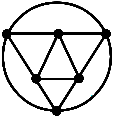
\includegraphics[width=1.7cm]{img/octaedro2.png} 
    & 
    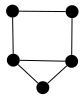
\includegraphics[width=1.5cm]{img/ex3.png} 
    & 
    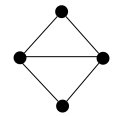
\includegraphics[width=2cm]{img/diamondNoLabel.png} 
    & 
    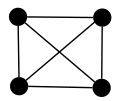
\includegraphics[width=1.5cm]{img/k4.png} 
    & 
    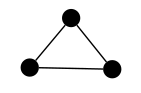
\includegraphics[width=2cm]{img/k3.png} 
    \\
    \footnotesize 
    (a)  \footnotesize Grafo $E_1$. 
    & 
    \footnotesize (b) Grafo $E_2$.
    & 
    \footnotesize (c) Grafo $E_3$.
    & 
    \footnotesize (d) Grafo $E_4$.
    & 
    \footnotesize (e) Grafo $E_5$.
    \\%%Segunda linha
        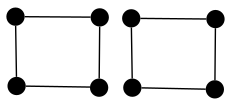
\includegraphics[width=2.5cm]{img/2c4.png} 
    & 
    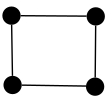
\includegraphics[width=1.5cm]{img/c4e.png} 
    & 
    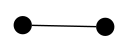
\includegraphics[width=1.8cm]{img/k2.png} 
    & 
    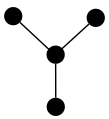
\includegraphics[width=1cm]{img/e10.png} 
    & 
    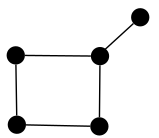
\includegraphics[width=1.8cm]{img/e11.png} 
    \\ %%Segundo Bloco legendas
    \footnotesize 
    (f)  \footnotesize Grafo $E_7$. 
    & 
    \footnotesize (g) Grafo $E_8$.
    & 
    \footnotesize (h) Grafo $E_9$.
    & 
    \footnotesize (i) Grafo $E_{10}$.
    & 
    \footnotesize (j) Grafo $E_{11}$.
    %%Terceira linha de imagens
    \\%%Terceira linha
        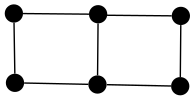
\includegraphics[width=2.5cm]{img/e12.png} 
    & 
    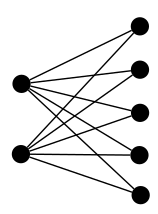
\includegraphics[width=2cm]{img/k25.png} 
    & 
    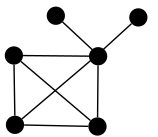
\includegraphics[width=2cm]{img/e14.png} 
    & 
    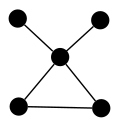
\includegraphics[width=1.8cm]{img/e15.png} 
    & 
    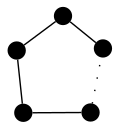
\includegraphics[width=1.8cm]{img/c2n+1.png} 
    \\ %%Terceiro Bloco legendas
    \footnotesize 
    (k)  \footnotesize Grafo $E_{12}$. 
    & 
    \footnotesize (l) Grafo $E_{13}$.
    & 
    \footnotesize (m) Grafo  $E_{14}$.
    & 
    \footnotesize (n) Grafo $E_{15}$.
    & 
    \footnotesize (o)  Grafo $E_{16}$,  $C_{2n+1},n\geq2$.
    \\
    &&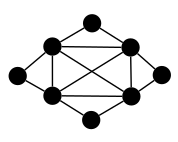
\includegraphics[width=2.5cm]{img/4sunNoLabel.png}&&
    \\
    &&\footnotesize (p)  Grafo $E_{17}$.&&
    
    %\multicolumn{3}{c}{ \footnotesize (c) Another partial single bend representation of $H$ } \\
  \end{tabular}
 \caption{O conjunto de instâncias para o diagrama de Venn das classes de grafos estudadas até aqui.}
 %, see  more in~\cite{leveque2009characterizing,tondato2009grafos}
 \label{fig:exemplosDiagram}
\end{figure}  
 